\documentclass[12pt,a4paper]{article}
\usepackage[utf8]{inputenc}
\usepackage[ukrainian]{babel}
\usepackage{amsmath}
\usepackage{amsfonts}
\usepackage{amssymb}
\usepackage{graphicx}
\usepackage{hyperref}
\usepackage[left=2cm,right=2cm,top=2cm,bottom=2cm]{geometry}

\begin{document}

\begin{titlepage}
    \centering
    \vspace*{1cm}

    \Large
    Київський національний університет імені Тараса Шевченка \\

    \vspace{0.5cm}

    \large
    Факультет комп'ютерних наук та кібернетики \\

    \vspace{0.5cm}

    Кафедра інтелектуальних інформаційних систем \\

    \vspace{0.5cm}

    Алгебро-автоматичні методи проектування програмного забезпечення \\

    \vspace{3cm}

    \textbf{Лабораторна робота 1} \\

    \vspace{0.5cm}

    "Скінченні автомати" \\

    \vspace{2cm}

    Виконали студенти 1-го курсу \\

    \vspace{0.2cm}

    Групи ПЗС-1 \\

    \vspace{0.1cm}

    Рябов Кирило \\

    \vspace{0.1cm}

    Соколов Михайло \\

    \vspace{0.1cm}

    Рибачок Руслан \\

    \vfill

    2023

\end{titlepage}

\section*{Лабораторна 1: Перетворення е-НДСА в НДСА}

\textbf{Мета:} Перетворити епсилон-недетермінований скінченний автомат (е-НДСА) на недетермінований скінченний автомат (НДСА).

\subsection*{Посилання на репозиторій з кодом:}

\href{https://github.com/KyrylR/Automata-1-2023-labs}{https://github.com/KyrylR/Automata-1-2023-labs}

\subsection*{Псевдокод:}

\begin{flalign*}
& \textbf{Вхід:} \quad \text{е-НДСА } A = (A, X, f, a_0, F) & \\
& \textbf{Вихід:} \quad \text{НДСА } B = (A', X, f', a_0', F') & \\
& \textbf{Кроки:} &
\end{flalign*}

\begin{enumerate}
    \item \textbf{Ініціалізуємо змінні для НДСА:}
    \begin{itemize}
        \item \( a_0' \): Встановлюємо рівним \( a_0 \).
        \item \( A' \): Ініціалізуємо з \( \{a_0'\} \).
        \item \( f' \): Ініціалізуємо порожньою множиною.
        \item \( F' \): Встановлюємо як \( F \cap a_0 \).
        \item \( f'' \): Ініціалізуємо порожньою множиною.
        \item \( W \): Встановлюємо як всі переходи, починаючи з \( a_0 \) у \( f \).
    \end{itemize}

    \item \textbf{Обробляємо кожен перехід у \( W \) доки \( W \) не порожній:}
    \begin{itemize}
        \item Вибраємо перехід \( (a_1, \alpha, a_2) \) з \( W \).
        \begin{enumerate}
            \item Якщо \( \alpha \) не належить \( epsilon \):
            \begin{itemize}
                \item Додаємо \( a_2 \) до \( A' \).
                \item Додаємо \( (a_1, \alpha, a_2) \) до \( f' \).
                \item Якщо \( a_2 \) в \( F \), додаємо \( a_2 \) до \( F' \).
                \item Для \( a_3 \), досягнутих \( epsilon \) з \( a_2 \):
                \begin{itemize}
                    \item Якщо \( (a_1, \alpha, a_3) \) не в \( f' \), додаємо до \( W \).
                \end{itemize}
                \item Для \( x \) в \( X \) та \( a_3 \) досягнутих \( x \) з \( a_2 \):
                \begin{itemize}
                    \item Якщо \( (a_2, x, a_3) \) не в \( f' \), додаємо до \( W \).
                \end{itemize}
            \end{itemize}
            \item Інакше:
            \begin{itemize}
                \item Додаємо \( (a_1, \alpha, a_2) \) до \( f'' \).
                \item Якщо \( a_2 \) в \( F \), додаємо \( a_0 \) до \( F' \).
                \item Для \( \beta \) в \( X \) об'єднання з \( epsilon \) та \( a_3 \) досягнутих \( \beta \) з \( a_2 \):
                \begin{itemize}
                    \item Якщо \( (a_1, \beta, a_3) \) не в \( f' \cup f'' \), додаємо до \( W \).
                \end{itemize}
            \end{itemize}
        \end{enumerate}
    \end{itemize}

    \item \textbf{Повернутаємо результуючий НДСА \( B \).}
\end{enumerate}

\newpage

\subsection*{Пояснення:}

Цей алгоритм має на меті перетворення е-НДСА на НДСА. Основна проблема полягає в обробці epsilon переходів.

\vspace{0.5em}
Результуючий НДСА матиме всі стани та переходи е-НДСА. Однак, додаткові переходи будуть додані на основі epsilon переходів в е-НДСА.
\vspace{0.5em}

Epsilon-переходи обробляються двома способами:
\begin{itemize}
    \item Додаючи переходи, що виникають з epsilon-переходів.
    \item Розглядаючи всі можливі стани, які можна досягти після виконання одного або декількох epsilon-переходів, та додаючи відповідні переходи до них у НДСА.
\end{itemize}

Алгоритм використовує робочу множину \( W \) для відстеження переходів, які потрібно обробити. Процес триває до тих пір, поки всі переходи не будуть враховані.

\subsection*{Складність алгоритму:}
Як випливає з наведених вище кроків, алгоритм має таку оцінку \( O(|A|^2|X||f|) \)

\subsection*{Результат роботи алгоритму:}

Алгоритм для перетворення е-НДСА на НДСА дозволяє нам ефективно обробляти epsilon-переходи та враховувати їх в результуючому НДСА. Це допомагає уникнути неоднозначності, яка може виникнути через присутність epsilon-переходів.

\vspace{1em}
\textbf{Приклад 1:}
\vspace{0.5em}

Розглянемо е-НДСА, який має наступні переходи:
\begin{itemize}
    \item \(0 \xrightarrow{x, \epsilon} 1\)
    \item \(1 \xrightarrow{y, \epsilon} 2\)
    \item \(2 \xrightarrow{z} 2\)
\end{itemize}

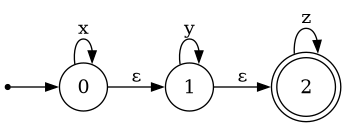
\includegraphics[width=0.5\textwidth]{e-nfa-automata_0.json.png}

Після застосування алгоритму перетворення отримаємо НДСА з такими переходами:
\begin{itemize}
    \item \(0 \xrightarrow{x} \{0, 1, 2\}\)
    \item \(0 \xrightarrow{y} \{1, 2\}\)
    \item \(0 \xrightarrow{z} 2\)
    \item \(1 \xrightarrow{y} \{1, 2\}\)
    \item \(2 \xrightarrow{z} 2\)
\end{itemize}

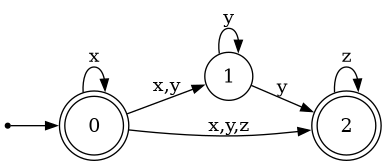
\includegraphics[width=0.5\textwidth]{nfa-automata_0.json.png}

Тут, як можна побачити, переходи, які були пов'язані з epsilon-переходами в е-НДСА, були успішно оброблені та додані до результуючого НДСА.

Here is the updated text for example 4:

\vspace{1em}
\textbf{Приклад 2:}
\vspace{0.5em}

Розглянемо результати обробки файлу \( automata\_1.json \). Оригінальний е-НДСА має наступну структуру:

\begin{itemize}
    \item \(1 \xrightarrow{e} \{2, 3\}\)
    \item \(2 \xrightarrow{a} 2\)
    \item \(2 \xrightarrow{b} 3\)
    \item \(3 \xrightarrow{c} 4\)
    \item \(3 \xrightarrow{e} 2\)
    \item \(4 \xrightarrow{a} 4\)
\end{itemize}

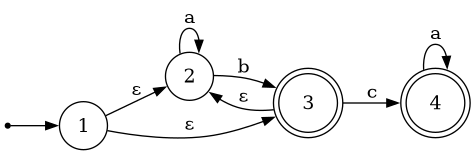
\includegraphics[width=0.5\textwidth]{e-nfa-automata_1.json.png}

Після застосування алгоритму перетворення отримаємо НДСА з такими переходами:
\begin{itemize}
    \item \(1 \xrightarrow{a} 2\)
    \item \(1 \xrightarrow{b} \{2, 3\}\)
    \item \(1 \xrightarrow{c} 4\)
    \item \(2 \xrightarrow{a} 2\)
    \item \(2 \xrightarrow{b} \{2, 3\}\)
    \item \(3 \xrightarrow{c} 4\)
    \item \(4 \xrightarrow{a} 4\)
\end{itemize}

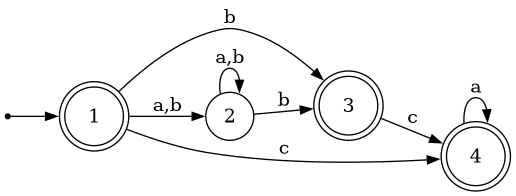
\includegraphics[width=0.5\textwidth]{nfa-automata_1.json.png}

В цьому прикладі цікаво спостерігати, як стан \(1\) стає кінцевим після перетворення, тому що він може досягти кінцевих станів \(3\) або \(4\) через epsilon-перехід.

\vspace{1em}
\textbf{Приклад 3:}
\vspace{0.5em}

Розглянемо результати обробки файлу \( automata\_2.json \). Оригінальний е-НДСА має наступну структуру:

\begin{itemize}
    \item \(1 \xrightarrow{b, e} 2\)
    \item \(1 \xrightarrow{e} 3\)
    \item \(2 \xrightarrow{b} 1\)
    \item \(3 \xrightarrow{a} 4\)
    \item \(3 \xrightarrow{b} 5\)
    \item \(4 \xrightarrow{a} 3\)
    \item \(5 \xrightarrow{a} 3\)
\end{itemize}

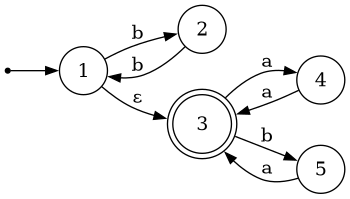
\includegraphics[width=0.5\textwidth]{e-nfa-automata_2.json.png}

Після застосування алгоритму перетворення отримаємо НДСА з такими переходами:
\begin{itemize}
    \item \(1 \xrightarrow{a} 4\)
    \item \(1 \xrightarrow{b} \{2, 5\}\)
    \item \(2 \xrightarrow{b} \{1, 3\}\)
    \item \(3 \xrightarrow{a} 4\)
    \item \(3 \xrightarrow{b} 5\)
    \item \(4 \xrightarrow{a} 3\)
    \item \(5 \xrightarrow{a} 3\)
\end{itemize}

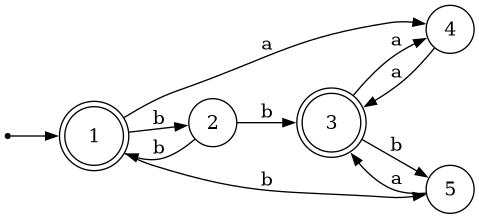
\includegraphics[width=0.5\textwidth]{nfa-automata_2.json.png}

В цьому прикладі цікаво спостерігати, як стан \(1\) стає кінцевим після перетворення, тому що він може досягти кінцевого стану \(3\) через epsilon-перехід.

\vspace{1em}
\textbf{Приклад 4:}
\vspace{0.5em}

Розглянемо результати обробки файлу \( automata\_3.json \). Оригінальний е-НДСА має наступну структуру:

\begin{itemize}
    \item \(1 \xrightarrow{b} 2\)
    \item \(1 \xrightarrow{c} 3\)
    \item \(1 \xrightarrow{e} \{2, 3\}\)
    \item \(2 \xrightarrow{a} 1\)
    \item \(2 \xrightarrow{b} 3\)
    \item \(2 \xrightarrow{c} \{1, 2\}\)
\end{itemize}

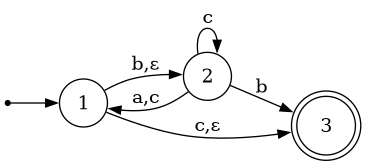
\includegraphics[width=0.5\textwidth]{e-nfa-automata_3.json.png}

Після перетворення отримаємо НДСА з такими переходами:
\begin{itemize}
    \item \(1 \xrightarrow{a} \{1, 2, 3\}\)
    \item \(1 \xrightarrow{b} \{2, 3\}\)
    \item \(1 \xrightarrow{c} \{1, 2, 3\}\)
    \item \(2 \xrightarrow{a} \{1, 2, 3\}\)
    \item \(2 \xrightarrow{b} 3\)
    \item \(2 \xrightarrow{c} \{1, 2, 3\}\)
\end{itemize}

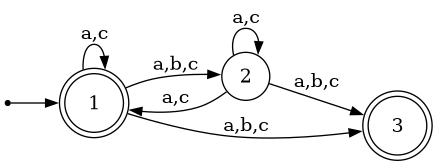
\includegraphics[width=0.5\textwidth]{nfa-automata_3.json.png}

В цьому прикладі цікаво спостерігати, як перетворення збільшило кількість кінцевих станів, тому що стан \(1\) може досягти кінцевого стану \(3\) через epsilon-перехід, і тому сам стає кінцевим.

\vspace{1em}
\textbf{Висновок:}
\vspace{0.5em}

Алгоритм надає нам засіб для перетворення е-НДСА на НДСА, враховуючи всі можливі стани, які можна досягти через epsilon-переходи. Результуючий НДСА є повністю визначеним і не містить epsilon-переходів, що спрощує його аналіз та використання. З цієї роботи ми навчилися основам роботи з е-НДСА і НДСА та перетворення одного в інший.


\end{document}
